\documentclass[12pt,oneside]{book}
\usepackage{fullpage}
\usepackage{color}
\usepackage{mathtools}
\usepackage{amsmath}
\usepackage{amsfonts}
\usepackage{graphicx}
\usepackage{lipsum}
\usepackage[utf8]{inputenc}
\usepackage{geometry}
\usepackage{fancyhdr}
 

\rfoot{Page \thepage}

\geometry{
 a4paper,
 total={210mm,297mm},
 left=35mm,
 right=25mm,
 top=25mm,
 bottom=25mm,
}
\linespread {1.6}

\newif\ifquoteopen
\catcode`\"=\active % lets you define `"` as a macro
\DeclareRobustCommand*{"}{%
   \ifquoteopen
     \quoteopenfalse ''%
   \else
     \quoteopentrue ``%
   \fi
}




%Gummi|065|=)

\date{}
\begin{document}

%% ----------------------------------------------PAGE 1 TITLE

\begin{titlepage}
    \begin{center}
        \vspace*{1cm}
        
        {\scshape {\huge{I}\Large{NTER-PROCEDURAL} \huge{A}\Large{NALYSIS OF}\\
                   \vspace{0.1cm}
				   \huge{C}\Large{ONCOLIC } \huge{E}\Large{XECUTION}}}\\[1.5cm] % Thesis title

        
        \textit{A Thesis Submitted\\
        in Partial Fulfilment of the Requirements\\
        for the Degree of\\}
                \vspace{0.8cm}
        \textbf{\large{MASTER OF TECHNOLOGY}}\\[0.5\baselineskip]
        \textit{by}\\[0.5\baselineskip]
        \textbf{\large{Ashwini Kshitij}}\\
                \vspace{0.8cm}
        \textit{supervised by}\\
                \vspace{0.8cm}
        \textbf{\large{Dr. Subhajit Roy}}\\
        \textbf{\large{Dr. Amey Karkare}}
        \vspace{0.8cm}
        
      	
\includegraphics[width=0.25\textwidth]{iitklogo.png}
        
        \vspace{1\baselineskip}
        
        \uppercase{Department of Computer Science and Engineering\\
        \textbf{Indian Institute of Technology Kanpur}}\\
        
        \vspace{1\baselineskip}
        \textbf{June 2015}
        
    \end{center}
\end{titlepage}


%%-----------------------------------------------PAGE 2 Certificate

\frontmatter
\addcontentsline{toc}{chapter}{Certificate}
\begin{center}
\textbf{\Large{CERTIFICATE}}
\end{center}
\vspace*{3\baselineskip}
This is to certify that the work contained in this thesis entitled \textbf{\textit{"Inter-procedural analysis of Concolic Execution"}}, by \textbf{Ashwini Kshitij (Roll No. 10327165)}, has been carried out under my supervision and this work has not been submitted elsewhere for a degree.\\
\\[4\baselineskip]

  \small
  \vspace{2.0 cm}
  \begin{tabular*}{1.0\textwidth}{@{\extracolsep{\fill}} l r}
    \textbf{Dr. Subhajit Roy} 			 & 				\textbf{Dr. Amey Karkare}\\
    Assistant Professor,				 &				Assistant Professor,\\
    Department of CSE, 					 & 				Department of CSE,\\
    IIT Kanpur.							 &				IIT Kanpur.
    
  \end{tabular*}
\newpage


%%----------------------------------------------ABSTRACT
\addcontentsline{toc}{chapter}{Abstract}
\begin{center}
\textbf{\Large{ABSTRACT}}
\end{center}
\vspace {0.8 cm}

Interprocedural analysis is the cornerstone of determining precise program behavioral information. Using this technique we can avoid making overly conversative assumptions about the effects of procedures and the state at call sites. It aims at gathering informations across multiple procedures.  

\vspace {0.5 cm}

In this thesis, to extend the concept of concolic execution to interprocedural calls we instrument the function call site. For such instrumentation purposes we have used a tool called CIL. Just before the function call we set up the environment for calling the procedure which in turn enables the it follow through the symbolic execution of parameters with the control flow from caller to callee. Similarly, just after the call instruction we restore the calling environment by restoring the symbolic values.

\vspace {0.5 cm}

Modifying the symbolic execution engine to collect the interprocedural analysis information can have widepread applications in software verification and testing. We can improve the coverage of test suites that are automatically generated by intraprocedural concolic executers.   

  






\newpage

%%----------------------------------------------ACKNOWLEDGMENT
\addcontentsline{toc}{chapter}{Acknowledgement}
\begin{center}
\textbf{\Large{Acknowledgements}}
\end{center}

\vspace{1.0 cm}

I acknowledge, with gratitude, my debt of thanks to Professor Subhajit Roy for his advise and encouragement and to Professor Amey Karkare for his aid and foresight. They presented me with the opportunity to tackle interesting problems in field of Software Testing. Their patient but firm guidance was critical to successful completion of my research.  

\vspace{0.5 cm}

I appreciate the support of my friends and wingmates who always provided me with the confidence and courage to tackle even the most challenging problems. Without their help and councel, the completion this work would have been immeasurably more difficult. 

\vspace{1.0 cm}

I also want to express my sincere gratitude to \textit {\textbf {BRNS}} for encouraging our research work. Their unshaken faith in our efforts motivated me to follow through this project.

\begin{flushright}
\textbf{-Ashwini Kshitij}
\end{flushright}

\newpage

%%----------------------------------------------CONTENTS

\tableofcontents
\mainmatter

%%---------------------------------------------CHAP 1 Intro

\chapter{Introduction}
%%\lhead{Chapter 1. \emph{Introduction}}


\hspace {0.4 cm}
Symbolic Execution has been a recipient of significant attention during the past few years. It is now considered an effective technique in generation of high coverage test suites. The idea has been discovered around three decades ago but it was after significant improvements the potential of idea is harnessed. One such important improvement was symbolic execution alongside keeping track of concrete values (concolic executic). The main advantage of this technique is that whenever constraint solving complications (like timeouts) occur during classical symbolic execution, it is alleviated using the concrete values.

More practical programs involve procedure calls. The symbolic execution goes smoothly if there are no function calls involve. A function call tranfers the control from the caller to the callee. That function may very well modify the symbolic state of the variables. If we transition the symbolic state correctly through the function call, the symbolic execution will run as usual with the modified symbolic state.   


\section{Problem Statement}
The implementation of this thesis is built into a tool 'Testgen' that does automatic test case generation. The tool uses inbuilt concolic execution engine for the purpose. But one of the drawbacks the tool faces is whenever a procedure call is encountered, the symbolic value is reset to "start state" instead of modifying it as per the operations performed on it by the callee function.  

\newpage

\begin{figure}[htbp]
\centering
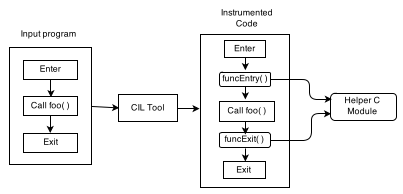
\includegraphics[scale=1]{module3.png}
\caption{Basic Module}
\end{figure}

\textit{Figure 1.1} shown above gives a vague idea of what the tool does. We are given a C program with a concolic execution engine integrated with it. Problem arises with execution when it comes across a procedure call instruction. The symbolic state of the input variables is set to default as the tool does not have the ability to follow through symbolic execution from caller to callee and then back to the caller.

We aim at solving this problem by instrumenting the call site. For such purposes in our approach we have used a tool called CIL. We first set up an environment before commencing the callee procedure execution (in this case \textit{foo}). The operations for such tasks is carried out by \textit{funcEntry} function which is instrumented just before \textit{foo} is called. \textit{funcEntry} handles the mapping of symbolic and concolic values of actual parameters to formal parameters, the creation of symbolic stack (later explained in \textit{Chapter 3}).

Similarly we instrument \textit{funcExit} function just after \textit{foo} call. The task of \textit{funcExit} is to map the symbolic state of "return variable" to appropriate variable at the call site (if any) and clear the symbolic values that were generated during call and execution of \textit{foo}. It also manages the symbolic stack appropriately. The implementation of \textit{funcEntry} and \textit{funcExit} is done in C language and is defined in included C modules.

This approach ensures that symbolic execution is carried through correctly to and from the callee. The modified state of symbolic variables is in accordance with operations of concerned callee function (in our case \textit{foo}). This improves the accuracy and correctness of the test suite generation in our tool.  

\section {Contributions}
In this thesis we have accomplished the following:
\begin{itemize}
  \item Designed an approach to apply inter-procedural analysis to concolic execution. 
  \item Application of IP analysis to improve the automatic test case generation using concolic testing.
  \item Dynamic support to handle recursive procedure calls. 
\end{itemize}


\section {Organisation of thesis}
A brief summary of the contents of other chapters of this thesis are as follows.\\

\textbf{Chapter 2} deals with the concepts which are necessary to understand the thesis. Concolic execution is introduced and its advantages over classical symbolic execution and random testing. Meaning of coverage and test suite generation is also explained. Some brief approaches in interprocedural analysis has also been discussed in this chapter. We also explore the related work that has been done in this field. \\

\textbf{Chapter 3} discusses our implementation in a detailed manner. Some terminology has been introduced to explain techniques employed in our work. But mostly the chapter pertains to the relevant algorithms designed to accomplish the aim of this thesis and how it should improve the scalability and accuracy of this tool.\\

\textbf{Chapter 4} contains the experimental results and their analysis after we run our modified tool on a set of standard benchmark programs. Analysis in done in terms of coverage improvement and runtime of the tool.\\

\textbf{Chapter 5} sheds light on future work and modifications that can be done to improve the accuracy and performance of the approach discussed in this thesis.


\newpage
\chapter{Background}

\section {Concolic Testing}

\section {Intraprocedural Analysis}
\newpage


\chapter{Methodology}



\end{document}
